\chapter{E/I Clustered Networks}
\label{ch:ei-clustered-networks}

The previous chapters built the language of attractors, stochastic spike trains,
balanced recurrent networks, clustered assemblies, random rate chaos, and
dynamic mean-field theory. This chapter puts those tools into the architecture
that motivates the research program: excitatory and inhibitory populations are
clustered together. The central idea is simple but powerful. A cluster is no
longer only a group of recurrently potentiated excitatory cells. It is a paired
excitatory-inhibitory module whose local excitation, local inhibition, and
inter-cluster disorder make it behave like an effective rate unit.

\section*{Learning Goals}

After this chapter you should be able to:
\begin{itemize}
    \item write the spike-train, population-activity, and filtered-current
    variables for a paired E/I clustered network;
    \item explain Tilo's \(J_E^+\), \(J_I^+\), \(R_J\) (also written \(R\)),
    \(\widehat J\), and \(\check J\) notation;
    \item distinguish finite-size fluctuations, controlled by
    \(\xi_E=1/\sqrt{n_E}\) for an excitatory cluster, from quenched
    inter-cluster variability, controlled by \(\kappa\);
    \item explain why clustered inhibitory structure can amplify quenched
    variability relative to an E-only clustered network.
\end{itemize}

\section{Why Cluster Inhibition?}
\label{sec:ch08-why-cluster-inhibition}

In an E-clustered network, excitatory neurons are divided into assemblies while
the inhibitory pool is homogeneous. Such networks can support many attractors:
one set of excitatory clusters is active, another is silent, and finite-size
spiking fluctuations eventually kick the system from one basin to another. This
mechanism is useful, but it has a diagnostic weakness. If the number of neurons
per cluster is sent to infinity while the number of clusters is fixed, the
finite-size kick disappears.

An E/I-clustered network changes the question. Each excitatory cluster is paired
with an inhibitory cluster. The cluster state is therefore not a scalar firing
rate but a two-population state,
\begin{equation}
    r_a(t) = \bigl(r_a^E(t), r_a^I(t)\bigr),
    \qquad a=1,\ldots,Q ,
    \label{eq:ch08-paired-rate-state}
\end{equation}
where \(Q\) is the number of paired clusters. The excitatory component can
activate the pair; the inhibitory component can stabilize, suppress, or
disinhibit other pairs. This makes the cluster closer to a self-coupled rate
unit in a random rate network than to a passive bump of excitation.

\begin{figure}[t]
    \centering
    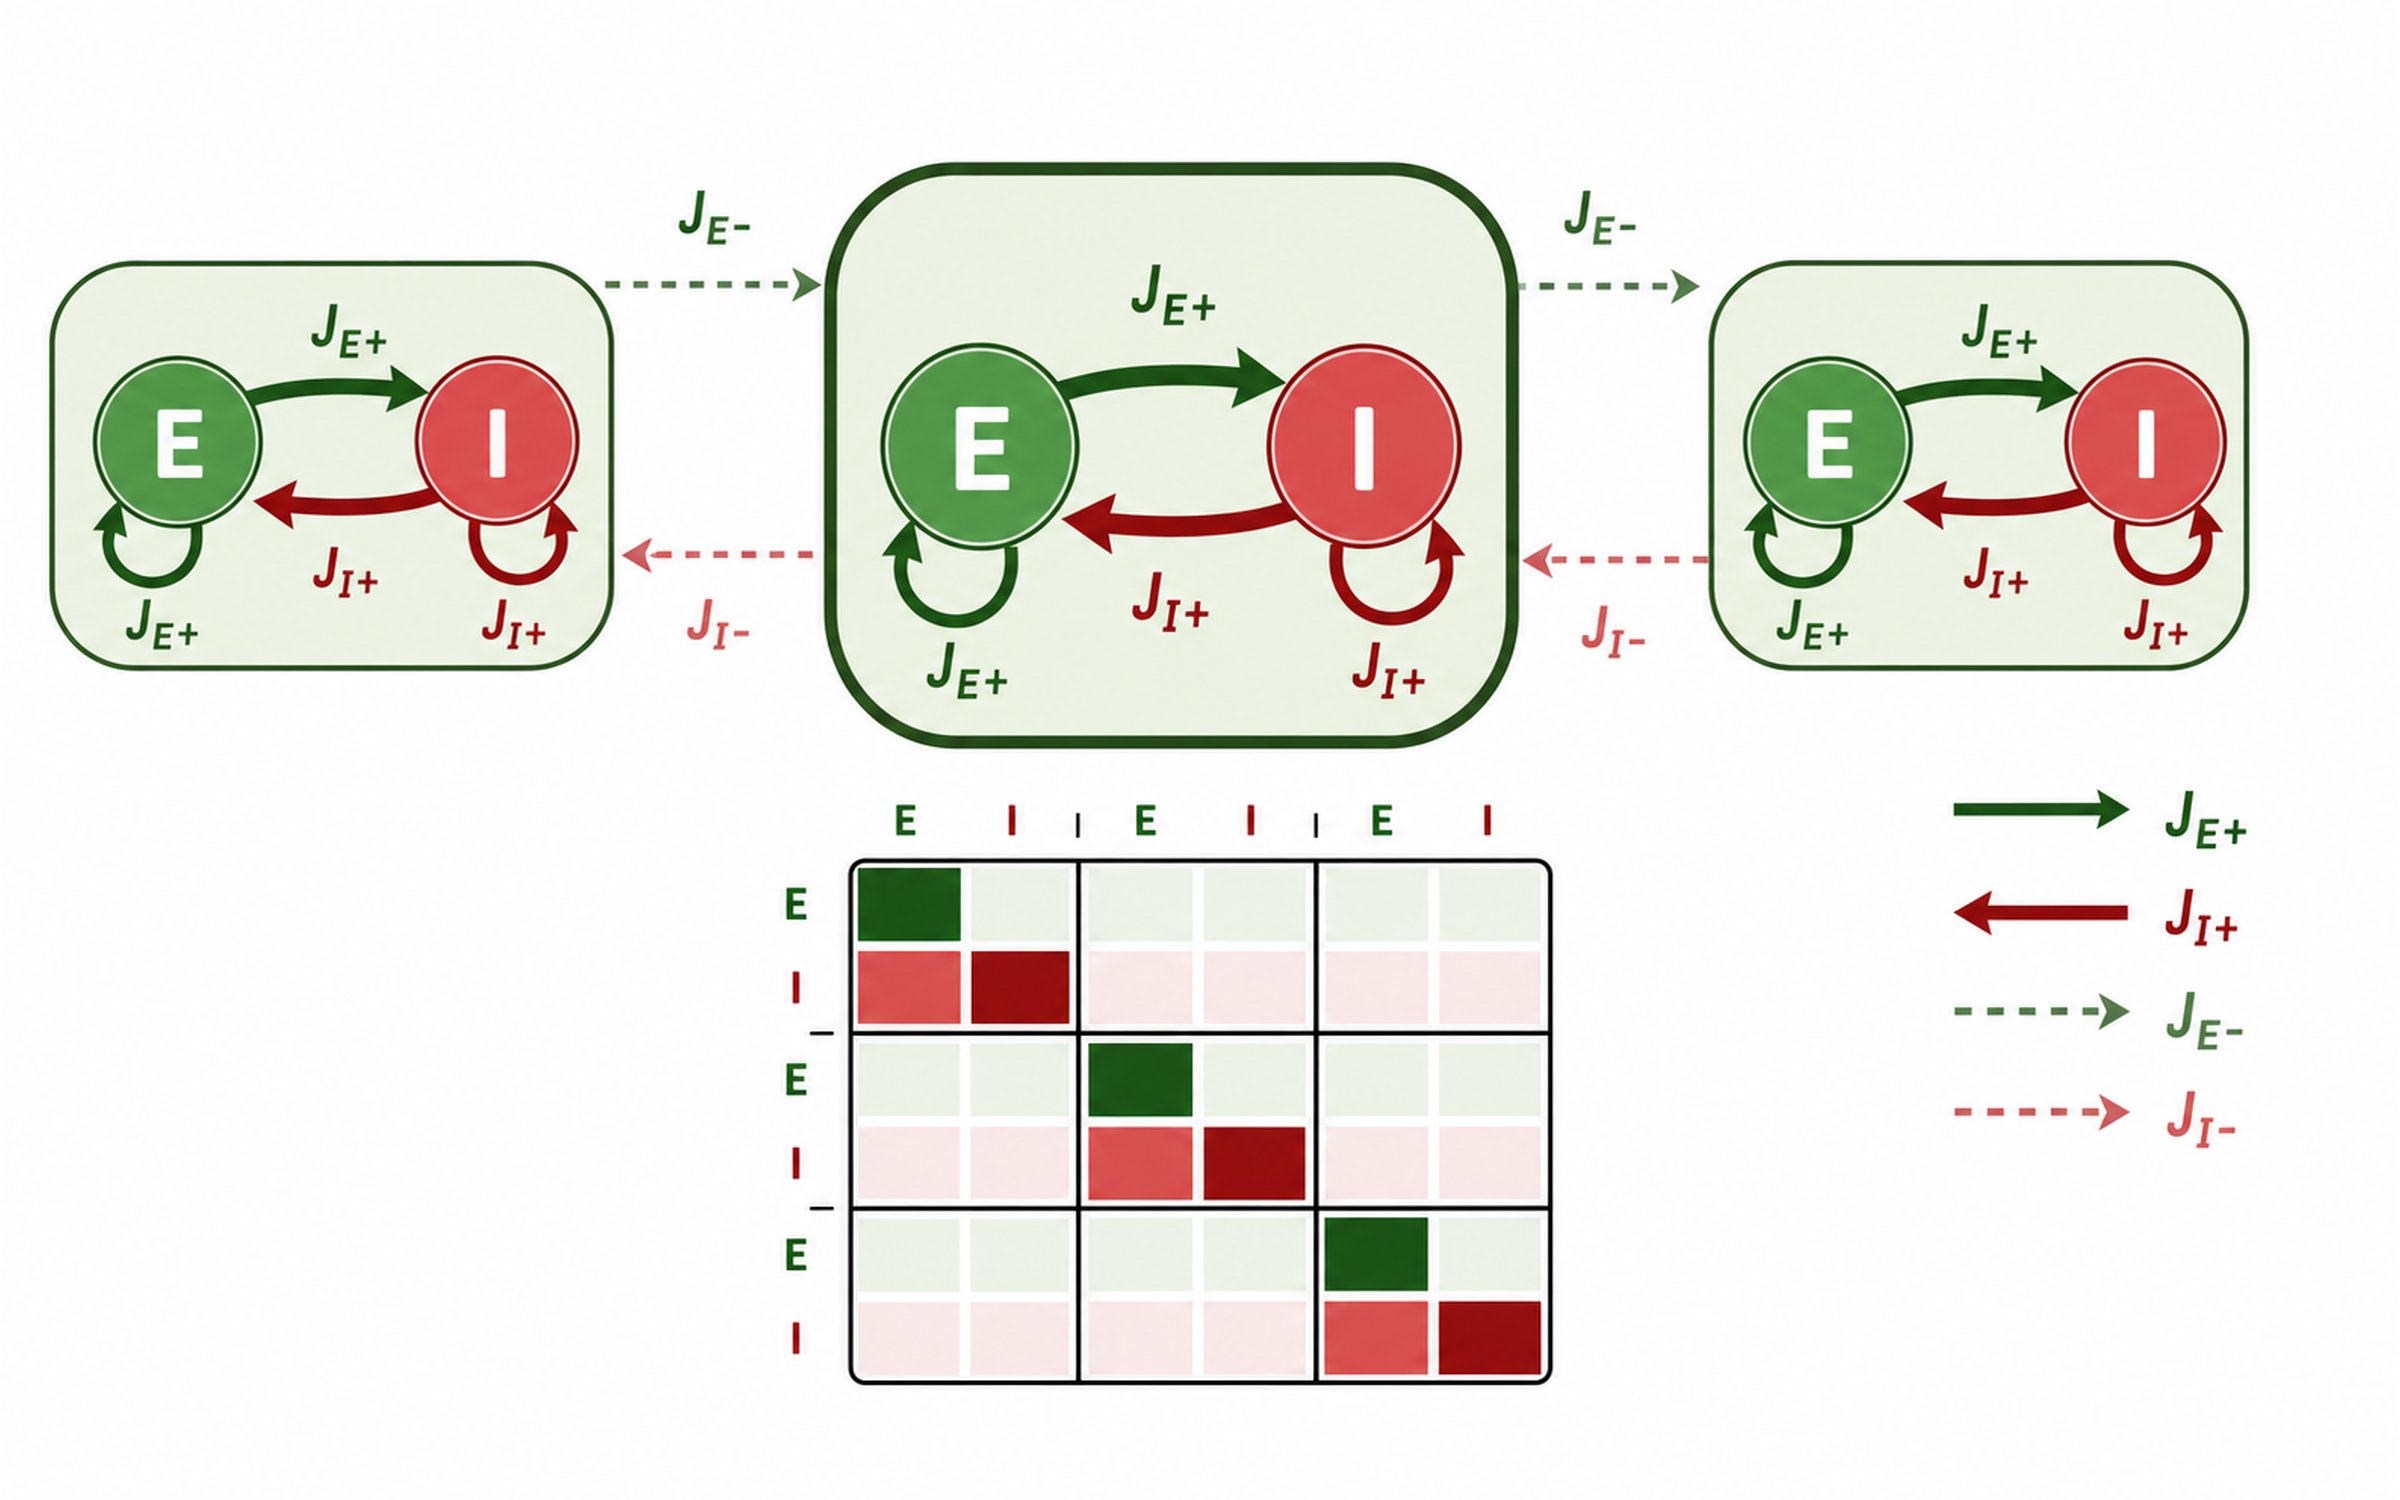
\includegraphics[width=0.92\textwidth]{figures/imagegen/ch08-paired-ei-clusters-img.png}
    \caption{A paired E/I cluster is a two-dimensional mesoscale unit. The EE
    connection within a pair is potentiated by \(J_E^+\), while the EI, IE, and
    II connections associated with the paired inhibitory population are
    potentiated by \(J_I^+\). Between distinct clusters the corresponding
    connections are depressed so that the mean recurrent drive can remain
    balanced.}
    \label{fig:ch08-paired-ei}
\end{figure}

\section{The Microscopic Variables}
\label{sec:ch08-microscopic-variables}

Use \(Q_E,Q_I\) for the numbers of excitatory and inhibitory clusters and
\(n_E,n_I\) for the number of neurons of each type inside one cluster. The
total class sizes are
\[
    N_E^{\mathrm{tot}}=Q_E n_E,\qquad
    N_I^{\mathrm{tot}}=Q_I n_I .
\]
The canonical paired E/I model sets \(Q_E=Q_I=Q\), pairs excitatory cluster
\(a\) with inhibitory cluster \(a\), and has
\begin{equation}
    N_c=n_E+n_I,
    \qquad
    N^{\mathrm{tot}}=Q(n_E+n_I),
    \qquad
    n_E=\gamma N_c,\quad
    n_I=(1-\gamma)N_c,
    \qquad 0<\gamma<1.
    \label{eq:ch08-fixed-ei-fractions}
\end{equation}
Thus a statement about increasing \(n_E\) is also a statement about increasing
\(N_c\), up to the fixed factor \(\gamma\). A spike train from neuron \(i\) of
type \(\alpha\in\{E,I\}\) in cluster \(a\) is
\begin{equation}
    s_{a,i}^{\alpha}(t)
    =
    \sum_k \delta\!\left(t-t_{a,i,k}^{\alpha}\right),
    \label{eq:ch08-spike-train}
\end{equation}
where \(t_{a,i,k}^{\alpha}\) is the time of the \(k\)-th spike. The population
activity is the empirical average
\begin{equation}
    A_a^\alpha(t)
    =
    \frac{1}{n_\alpha}
    \sum_{i=1}^{n_\alpha} s_{a,i}^{\alpha}(t),
    \qquad n_\alpha\in\{n_E,n_I\}.
    \label{eq:ch08-population-activity}
\end{equation}
This is still a point process. A firing-rate trace is obtained by filtering it
with a synaptic or analysis kernel. If
\begin{equation}
    \epsilon(t)=\frac{1}{\tau_s}e^{-t/\tau_s}\Theta(t),
\end{equation}
then the filtered synaptic current into a neuron in population \(\alpha\) of
cluster \(a\) is
\begin{equation}
    I_a^\alpha(t)
    =
    \int_{-\infty}^{t}
    \epsilon(t-t')\,y_a^\alpha(t')\,dt'.
    \label{eq:ch08-filtered-current}
\end{equation}
The unfiltered drive \(y_a^\alpha(t)\) is the signed weighted sum of spikes
arriving from inside and outside the cluster. The notation distinguishes
intra-cluster weights \(\widehat J^{\alpha\beta}\) from inter-cluster weights
\(\check J_{ab}^{\alpha\beta}\):
\begin{equation}
\begin{aligned}
    y_a^\alpha(t)
    &=
    \sum_{\beta\in\{E,I\}}
    \sum_{j=1}^{n_\beta}
    \widehat J^{\alpha\beta} s_{a,j}^{\beta}(t)
    \\
    &\quad+
    \sum_{b\ne a}
    \sum_{\beta\in\{E,I\}}
    \sum_{j=1}^{n_\beta}
    \check J_{ab}^{\alpha\beta} s_{b,j}^{\beta}(t).
\end{aligned}
\label{eq:ch08-microscopic-drive}
\end{equation}
The first index \(\alpha\) denotes the postsynaptic population and the second
index \(\beta\) denotes the presynaptic population. Thus \(J^{EI}\) means input
from inhibitory cells to excitatory cells, while \(J^{IE}\) means input from
excitatory cells to inhibitory cells.

At the population level, \cref{eq:ch08-microscopic-drive} becomes
\begin{equation}
    y_a^\alpha(t)
    =
    \sum_{\beta}
    \widehat J^{\alpha\beta} n_\beta A_a^\beta(t)
    +
    \sum_{b\ne a}
    \sum_{\beta}
    \check J_{ab}^{\alpha\beta} n_\beta A_b^\beta(t).
    \label{eq:ch08-population-drive}
\end{equation}
This equation is the bridge between the spiking network and the mesoscale
description. It says that a cluster is a rate unit only after the spikes have
been averaged over a population and filtered through synapses.

If the stationary population rates are homogeneous,
\(\langle A_a^\alpha(t)\rangle=r_\alpha\), then the mean input is
\begin{equation}
    \overline y_a^\alpha
    =
    \sum_{\beta}
    n_\beta r_\beta
    \left(
        \widehat J^{\alpha\beta}
        +
        \sum_{b\ne a}\check J_{ab}^{\alpha\beta}
    \right).
    \label{eq:ch08-stationary-mean-input}
\end{equation}
In a balanced parameterization the large positive excitatory part and the large
negative inhibitory part cancel, leaving a net input of the size needed to keep
neurons near threshold. The same decomposition gives the current
autocorrelation. At this level the formula is only schematic: it says how
population activity correlations are weighted by the recurrent couplings before
we impose the fixed in-degree construction used in the roadmap. If different
presynaptic clusters are asymptotically independent, then
\begin{equation}
    C_y^\alpha(\tau)
    \approx
    \sum_{\beta}
    n_\beta^2
    \left[
        \left(\widehat J^{\alpha\beta}\right)^2
        +
        \sum_{b\ne a}
        \left(\check J_{ab}^{\alpha\beta}\right)^2
    \right]
    C_A^\beta(\tau),
    \label{eq:ch08-current-autocorrelation}
\end{equation}
where \(C_A^\beta(\tau)\) is the autocorrelation of a population activity. A
dynamic mean-field closure asks for self-consistency: the autocorrelation
generated by a representative filtered input \(y(t)\) must reproduce the
population autocorrelation used to define that input.

The sparse fixed-indegree special case makes the balance cancellation explicit.
Use the reduced population-pair weights
\begin{equation}
    \widehat J^{\alpha E}=\widehat J,
    \qquad
    \widehat J^{\alpha I}=-g\widehat J,
    \qquad
    \check J_{ab}^{\alpha E}=\check J\Gamma_{ab}^{\alpha E},
    \qquad
    \check J_{ab}^{\alpha I}=-\check g\check J\Gamma_{ab}^{\alpha I}.
    \label{eq:ch08-fixed-degree-weights}
\end{equation}
Each target population receives exactly \(K_E=fK\) excitatory and
\(K_I=(1-f)K\) inhibitory source populations from other clusters, with
\(K\ll Q\):
\begin{equation}
    \sum_{b\ne a}\Gamma_{ab}^{\alpha E}=fK,
    \qquad
    \sum_{b\ne a}\Gamma_{ab}^{\alpha I}=(1-f)K .
    \label{eq:ch08-fixed-degree-row-sums}
\end{equation}
The inhibitory gain is chosen as
\begin{equation}
    \check g=\frac{fg}{1-f}.
    \label{eq:ch08-fixed-degree-gcheck}
\end{equation}
Then the population drive is
\begin{equation}
\begin{aligned}
    y_a^\alpha(t)
    &=
    \widehat J
    \left[
        n_E A_a^E(t)-g n_I A_a^I(t)
    \right]
    \\
    &\quad+
    \check J
    \sum_{b\ne a}
    \left[
        \Gamma_{ab}^{\alpha E}n_E A_b^E(t)
        -
        \check g\Gamma_{ab}^{\alpha I}n_I A_b^I(t)
    \right].
\end{aligned}
\label{eq:ch08-fixed-degree-drive}
\end{equation}
In this fixed-degree balance subsection, \(g\) and \(\check g\) are inhibitory
balance gains: they set the magnitude of inhibitory currents relative to
excitatory currents. They are not heterogeneity parameters. Quenched
inter-cluster heterogeneity will be denoted by \(\kappa\), with channel-specific
standard deviations written as \(\sigma_{\alpha\beta}^{\mathrm{het}}\).
If \(A_a^E\) and \(A_a^I\) have the same stationary rate \(r\), the choice
\(\check g=fg/(1-f)\) makes the outside-cluster mean proportional to the same
balanced difference as the inside-cluster mean:
\begin{equation}
    \overline y^\alpha
    =
    \left(\widehat J+\check J fK\right)
    \left(n_E-g n_I\right)r .
    \label{eq:ch08-fixed-degree-mean}
\end{equation}
Thus the cancellation is not an informal statement. The inhibitory in-degree
\((1-f)K\) and the factor \(\check g\) combine to give an inter-cluster
inhibitory mean \(-\check J fK\,g\,n_I r\), matching the excitatory coefficient
\(\check J fK\,n_E r\).

For second-order statistics, take \(Q\to\infty\) so that distinct cluster
activities are independent, and write a common population autocorrelation
\(C_A(\tau)\). The roadmap fixed in-degree calculation gives
\begin{equation}
    C_y^\alpha(\tau)
    =
    \left\{
        \widehat J^2\left(n_E^2+g^2n_I^2\right)
        +
        \check J^2 fK
        \left[
            n_E^2+\frac{g^2 f}{1-f}n_I^2
        \right]
    \right\}
    C_A(\tau).
    \label{eq:ch08-fixed-degree-autocorrelation}
\end{equation}
The first bracket is the paired-cluster contribution. The second bracket is
the inter-cluster contribution after summing \(fK\) excitatory inputs and
\((1-f)K\) inhibitory inputs with \(\check g=fg/(1-f)\). For large \(K\), the
inside-cluster term is subdominant and the simplified form is
\begin{equation}
    C_y^\alpha(\tau)
    \simeq
    \check J^2 fK
    \left[
        n_E^2+\frac{g^2 f}{1-f}n_I^2
    \right]
    C_A(\tau).
    \label{eq:ch08-large-k-autocorrelation}
\end{equation}
This is why sparse inter-cluster statistics cannot be treated as decorative:
in the large-\(K\) regime they dominate the input autocorrelation that the
dynamic mean-field closure must reproduce.

\section{Tilo's Cluster-Strength Notation}
\label{sec:ch08-tilo-notation}

Start from a balanced random E/I network with baseline signed synaptic weights
\(J_{EE},J_{EI},J_{IE},J_{II}\), where the second index is presynaptic and
\(J_{\alpha E}>0\), \(J_{\alpha I}<0\). The baseline weights are chosen so that
the large excitatory and inhibitory currents cancel to leave an \(O(1)\) net
input. Cluster structure is then introduced by multiplying within-pair
connections by potentiation factors and compensating between-pair connections
by depression factors.

For a paired E/I cluster, the roadmap notation uses an excitatory clustering
strength \(J_E^+\) and an inhibitory clustering strength \(J_I^+\). The simplest
version is
\begin{equation}
\begin{aligned}
    \widehat J^{EE} &= J_E^+ J_{EE},\\
    \widehat J^{EI} &= J_I^+ J_{EI},\\
    \widehat J^{IE} &= J_I^+ J_{IE},\\
    \widehat J^{II} &= J_I^+ J_{II}.
\end{aligned}
\label{eq:ch08-intra-potentiation}
\end{equation}
The first line strengthens recurrent excitation inside the excitatory assembly.
The last three lines say that, once inhibition is paired with the excitatory
assembly, the inhibitory loop is also locally structured. In simulations one
may choose separate factors for the four motifs, but equation
\cref{eq:ch08-intra-potentiation} is the reduced parameterization that exposes
the mechanism.

The inhibitory clustering strength is often tied to the excitatory one by
\begin{equation}
    J_I^+ = 1 + R_J\left(J_E^+ - 1\right).
    \label{eq:ch08-inhibitory-strength}
\end{equation}
Here \(R_J\) is the proportionality parameter called \(R\) in some roadmap
notes. If \(R_J=0\), the inhibitory population is effectively unclustered even
though the excitatory population is clustered. If \(R_J=1\), excitation and
inhibition are clustered with equal multiplicative strength. Intermediate
values express the useful case where inhibitory clusters exist but are weaker
than excitatory clusters. A value such as \(R_J=0.75\) should be treated as a
simulation setting when it appears in a specific implementation, not as a
universal constant.

The depression factors keep the mean recurrent input from changing just because
within-cluster connections were potentiated. If all \(Q\) clusters have equal
size, a row-average preserving choice is
\begin{equation}
    J_E^- = \frac{Q-J_E^+}{Q-1},
    \qquad
    J_I^- = \frac{Q-J_I^+}{Q-1}.
    \label{eq:ch08-depression-factors}
\end{equation}
To see why, average the multiplicative factor over one within-cluster target
and \(Q-1\) between-cluster targets:
\begin{equation}
    \frac{1}{Q}\left(J_E^+ + (Q-1)J_E^-\right)=1.
\end{equation}
The same identity holds for \(J_I^-\). Thus potentiation redistributes synaptic
strength across cluster pairs instead of simply increasing the total recurrent
gain. This is the dense equal-size template; in sparse fixed-indegree graphs one
must state whether the same dense factors are used on selected edges, or whether
the selected off-diagonal weights are renormalized to preserve the sparse row
sum.

With sparse inter-cluster connectivity, the depression factors are combined
with adjacency variables \(\Gamma_{ab}^{\alpha\beta}\). A schematic inter-cluster
weight is
\begin{equation}
    \check J_{ab}^{\alpha\beta}
    =
    D_{\alpha\beta}^{-} J_{\alpha\beta}\Gamma_{ab}^{\alpha\beta},
    \qquad a\ne b,
    \label{eq:ch08-intercluster-weight}
\end{equation}
where
\begin{equation}
    D_{EE}^{-}=J_E^-,
    \qquad
    D_{EI}^{-}=D_{IE}^{-}=D_{II}^{-}=J_I^- .
    \label{eq:ch08-depression-motifs}
\end{equation}
This convention matches the reduced paired-cluster parameterization:
inter-cluster EE connections use the excitatory depression factor, while EI,
IE, and II motifs use the inhibitory-pair depression factor. The binary matrix
\(\Gamma_{ab}^{\alpha\beta}\) records whether population \((b,\beta)\) projects
to population \((a,\alpha)\). In a fixed in-degree construction each population
receives \(K_E=fK\) excitatory and \(K_I=(1-f)K\) inhibitory cluster inputs, with
\(K\ll Q\). The inhibitory scaling can be chosen so that the mean excitatory and
inhibitory inter-cluster contributions cancel.

For the microscopic template below, separate two counts. Let
\(k_{ab}^{\alpha\beta}\) be the number of type-\(\beta\) presynaptic cells drawn
from one present population-pair block \((b,\beta)\to(a,\alpha)\). Let
\begin{equation}
    K_{\alpha\beta}^{\mathrm{eff}}(a)
    =
    \sum_{b:\,\Gamma_{ab}^{\alpha\beta}=1\ \mathrm{or}\ b=a}
    k_{ab}^{\alpha\beta}
    \label{eq:ch08-effective-cell-indegree}
\end{equation}
be the total type-\(\beta\) cell indegree across the local block and all selected
external blocks for one postsynaptic population. With equal allocation,
\(k_{ab}^{\alpha E}=k_{\alpha E}^{\mathrm{blk}}\) gives
\(K_{\alpha E}^{\mathrm{eff}}=(1+K_E)k_{\alpha E}^{\mathrm{blk}}\), and
\(k_{ab}^{\alpha I}=k_{\alpha I}^{\mathrm{blk}}\) gives
\(K_{\alpha I}^{\mathrm{eff}}=(1+K_I)k_{\alpha I}^{\mathrm{blk}}\).

\begin{keyequation}[Canonical Microscopic Weight Template]
\begin{equation}
    J_{i_a^\alpha,j_b^\beta}
    =
    C_{i_a^\alpha,j_b^\beta}\,
    \frac{j_{\alpha\beta}}{\sqrt{K_{\alpha\beta}^{\mathrm{eff}}(a)}}\,
    D_{ab}^{\alpha\beta}\,
    Z_{ab}^{\alpha\beta}.
    \label{eq:ch08-canonical-microscopic-weight}
\end{equation}
\begin{equation}
    D_{ab}^{\alpha\beta}
    =
    \begin{cases}
      J_E^+, & a=b,\ (\alpha,\beta)=(E,E),\\
      J_I^+, & a=b,\ (\alpha,\beta)\in\{(E,I),(I,E),(I,I)\},\\
      J_E^-, & a\ne b,\ (\alpha,\beta)=(E,E),\\
      J_I^-, & a\ne b,\ (\alpha,\beta)\in\{(E,I),(I,E),(I,I)\}.
    \end{cases}
    \label{eq:ch08-canonical-multipliers}
\end{equation}
\tcblower
\(C_{i_a^\alpha,j_b^\beta}\in\{0,1\}\) is the neuron-level adjacency inside an
allowed population-pair block, \(K_{\alpha\beta}^{\mathrm{eff}}(a)\) is the
total type-\(\beta\) cell indegree across all present blocks into one
postsynaptic type-\(\alpha\) neuron, \(j_{\alpha E}>0\) and \(j_{\alpha I}<0\)
are baseline signed amplitudes, \(D_{ab}^{\alpha\beta}\) implements
potentiation/depression, and \(Z_{ab}^{\alpha\beta}\) is a sign-preserving
quenched multiplier. Dividing by the total effective indegree keeps the
recurrent scale tied to the total number of sampled cells. If a simulator
instead divides by the per-block count \(k_{ab}^{\alpha\beta}\), then the
baseline amplitude \(j_{\alpha\beta}\) must be divided by the square root of the
number of present blocks in the equal-allocation case, or the recurrent scale
changes when \(K_E\) or \(K_I\) changes. If blocks
are dense rather than fixed cell-indegree, replace the denominator by the
scaling used by the target simulator, for example \(n_\beta\) for
rate-normalized blocks or \(\sqrt{N^{\mathrm{tot}}}\) for classical balanced
scaling with matching external drive.
\end{keyequation}

A convenient heterogeneity template is
\begin{equation}
    Z_{ab}^{\alpha\beta}
    =
    \begin{cases}
      1, & a=b,\\
      1+\kappa\sigma_{\alpha\beta}^{\mathrm{het}}G_{ab}^{\alpha\beta},
      & a\ne b,
    \end{cases}
    \qquad
    \langle G_{ab}^{\alpha\beta}\rangle=0,\quad
    \operatorname{Var}(G_{ab}^{\alpha\beta})=1 .
    \label{eq:ch08-weight-heterogeneity-template}
\end{equation}
For signed E/I weights, \(Z_{ab}^{\alpha\beta}\) should not flip the sign of
the synapse. One may resample negative multipliers, clip them, or use a
log-normal multiplier with matched mean and variance; the choice is an
implementation convention and should be recorded with the simulation seed.
After microscopic weights are aggregated into mesoscale couplings
\(W_{ab}^{\alpha\beta}\), the corresponding block-level standard deviation is
written \(\sigma_{\alpha\beta}^{W}\) below. It depends on the microscopic weight
scale, the cell-indegree allocation, and the multiplier variance
\(\sigma_{\alpha\beta}^{\mathrm{het}}\).

\begin{center}
\renewcommand{\arraystretch}{1.35}
\begin{tabularx}{\textwidth}{@{}l l X@{}}
  \toprule
  \textbf{Model component} & \textbf{Symbols} & \textbf{Canonical template choice} \\
  \midrule
  Paired architecture &
  \(Q_E,Q_I,n_E,n_I\) &
  Set \(Q_E=Q_I=Q\), pair E and I clusters by common label \(a\), and hold
  \(n_E/N_c=\gamma\) fixed in size sweeps. \\
  Baseline balance &
  \(j_{\alpha\beta},I_\alpha^{\mathrm{ext}}\) &
  Choose signed E/I weights and external drive from the balanced random network
  before adding cluster multipliers. \\
  Cluster multipliers &
  \(J_E^+,J_I^+,J_E^-,J_I^-\) &
  Potentiate within-pair EE by \(J_E^+\), within-pair EI/IE/II by \(J_I^+\),
  and depress off-diagonal blocks with the stated mean-preserving convention. \\
  Sparse source graph &
  \(\Gamma_{ab}^{\alpha\beta},K_E,K_I\) &
  For each target population, choose exactly \(K_E=fK\) E source clusters and
  \(K_I=(1-f)K\) I source clusters outside the paired cluster. \\
  Quenched disorder &
  \(\kappa,\sigma_{\alpha\beta}^{\mathrm{het}},\sigma_{\alpha\beta}^{W}\) &
  Draw one frozen multiplier per source-target cluster pair and channel; keep it
  fixed for all neurons in that block and for the whole simulation; record the
  induced aggregate-coupling variance. \\
  Rate extraction &
  \(\Delta t,\tau_f\) &
  Bin spikes into \(\widehat A_{a,m}^\alpha\), then filter with
  \cref{eq:ch08-filtered-rate-recursion}. \\
  \bottomrule
\end{tabularx}
\end{center}

\section{Network Generation Template}
\label{sec:ch08-network-generation-template}

The following is an implementable template, not a claim about one exact
published code path.
\begin{enumerate}
    \item Choose \(Q,n_E,n_I\), baseline signed amplitudes
    \(j_{\alpha\beta}\), total effective cell indegrees
    \(K_{\alpha\beta}^{\mathrm{eff}}\) or per-block allocations
    \(k_{ab}^{\alpha\beta}\), cluster-level source counts \(K_E=fK\) and
    \(K_I=(1-f)K\), potentiation \(J_E^+\), relative inhibitory clustering
    \(R_J\), and heterogeneity amplitudes
    \(\kappa\sigma_{\alpha\beta}^{\mathrm{het}}\).
    \item Assign neuron labels \((a,\alpha,i)\) with
    \(a=1,\ldots,Q\), \(\alpha\in\{E,I\}\), and
    \(i=1,\ldots,n_\alpha\). The paired local population of \((a,E)\) is
    \((a,I)\).
    \item Compute \(J_I^+=1+R_J(J_E^+-1)\) and the chosen depression factors
    \(J_E^-,J_I^-\). Dense equal-size factors use
    \cref{eq:ch08-depression-factors}; sparse-row factors should state their
    own row-sum convention.
    \item For each target population \((a,\alpha)\), set the local
    population-pair blocks \((a,E)\to(a,\alpha)\) and
    \((a,I)\to(a,\alpha)\) as present. Then draw exactly \(K_E\) external
    excitatory source clusters and exactly \(K_I\) external inhibitory source
    clusters without replacement to define
    \(\Gamma_{ab}^{\alpha E}\) and \(\Gamma_{ab}^{\alpha I}\).
    \item For every present population-pair block
    \((b,\beta)\to(a,\alpha)\), instantiate neuron-level adjacencies
    \(C_{i_a^\alpha,j_b^\beta}\). With fixed cell indegree, allocate
    \(k_{ab}^{\alpha\beta}\) presynaptic cells to each present block so that
    their sum equals \(K_{\alpha\beta}^{\mathrm{eff}}(a)\). Each target neuron
    then draws those cells from the source population without replacement,
    excluding self-connections when the source and target population are
    identical.
    \item Assign weights with
    \cref{eq:ch08-canonical-microscopic-weight}; draw and store
    \(Z_{ab}^{\alpha\beta}\) once per source-target cluster pair so the
    heterogeneity is quenched across time and shared by all neuron pairs in the
    block.
\end{enumerate}

\section{Clusters as Effective Rate Units}
\label{sec:ch08-effective-rate-units}

The cluster-level variable is not the instantaneous spike train but the binned
and filtered population rate. For half-open bins from \(t_m\) to
\(t_m+\Delta t\), define the spike count and empirical rate by
\begin{equation}
    C_{a,m}^\alpha
    =
    \sum_{i=1}^{n_\alpha}
    \int_{t_m}^{t_m+\Delta t}s_{a,i}^{\alpha}(u)\,du,
    \qquad
    \widehat A_{a,m}^{\alpha}
    =
    \frac{C_{a,m}^{\alpha}}{n_\alpha\Delta t}.
    \label{eq:ch08-binned-cluster-rate}
\end{equation}
For an exponential analysis filter with time constant \(\tau_f\), the discrete
recursion
\begin{equation}
    r_{a,m}^{\alpha}
    =
    e^{-\Delta t/\tau_f}r_{a,m-1}^{\alpha}
    +
    \left(1-e^{-\Delta t/\tau_f}\right)\widehat A_{a,m}^{\alpha}
    \label{eq:ch08-filtered-rate-recursion}
\end{equation}
implements the continuous convolution
\begin{equation}
    r_a^\alpha(t)
    =
    \int_{-\infty}^{t}
    h(t-t') A_a^\alpha(t')\,dt'.
    \label{eq:ch08-filtered-rate}
\end{equation}
The pair \((r_a^E,r_a^I)\) is an effective rate unit when its future is well
predicted by the collection of cluster rates and the fixed realization of
inter-cluster connectivity.

A schematic mesoscale reduction has the form
\begin{equation}
    \tau_\alpha \frac{d r_a^\alpha}{dt}
    =
    -r_a^\alpha
    +
    \Phi_\alpha\!\left(
        \sum_{\beta}
        W_{aa}^{\alpha\beta} r_a^\beta
        +
        \sum_{b\ne a}\sum_{\beta}
        W_{ab}^{\alpha\beta} r_b^\beta
        +
        I_{\alpha}^{\mathrm{ext}}
    \right)
    +
    \xi_\alpha B_\alpha(r_a^\alpha)\eta_a^\alpha(t).
    \label{eq:ch08-mesoscale-rate}
\end{equation}
The transfer function \(\Phi_\alpha\) summarizes the single-neuron response to
its filtered input. The matrix \(W_{aa}^{\alpha\beta}\) contains the
potentiated within-pair interactions. The matrices \(W_{ab}^{\alpha\beta}\)
contain depressed, random, or heterogeneous inter-pair interactions. The last
term represents finite-size fluctuations in the empirical population rate. The
prefactor \(B_\alpha\) depends on the point-process and filtering convention;
for a Poisson bin-count approximation its square is proportional to the local
rate. The size coordinate is
\begin{equation}
    \xi_\alpha = \frac{1}{\sqrt{n_\alpha}},
    \qquad
    \xi_E = \frac{1}{\sqrt{n_E}},
    \label{eq:ch08-xi}
\end{equation}
up to constants determined by rates and time bins. Under the fixed-fraction
convention in \cref{eq:ch08-fixed-ei-fractions},
\[
    \xi_E=(\gamma N_c)^{-1/2}\propto N_c^{-1/2}.
\]
The \(1/\sqrt{n_E}\) law is the central scaling: averaging over more excitatory
cells inside a cluster, equivalently over a larger paired cluster at fixed
\(\gamma\), suppresses sampling noise.

\begin{figure}[t]
    \centering
    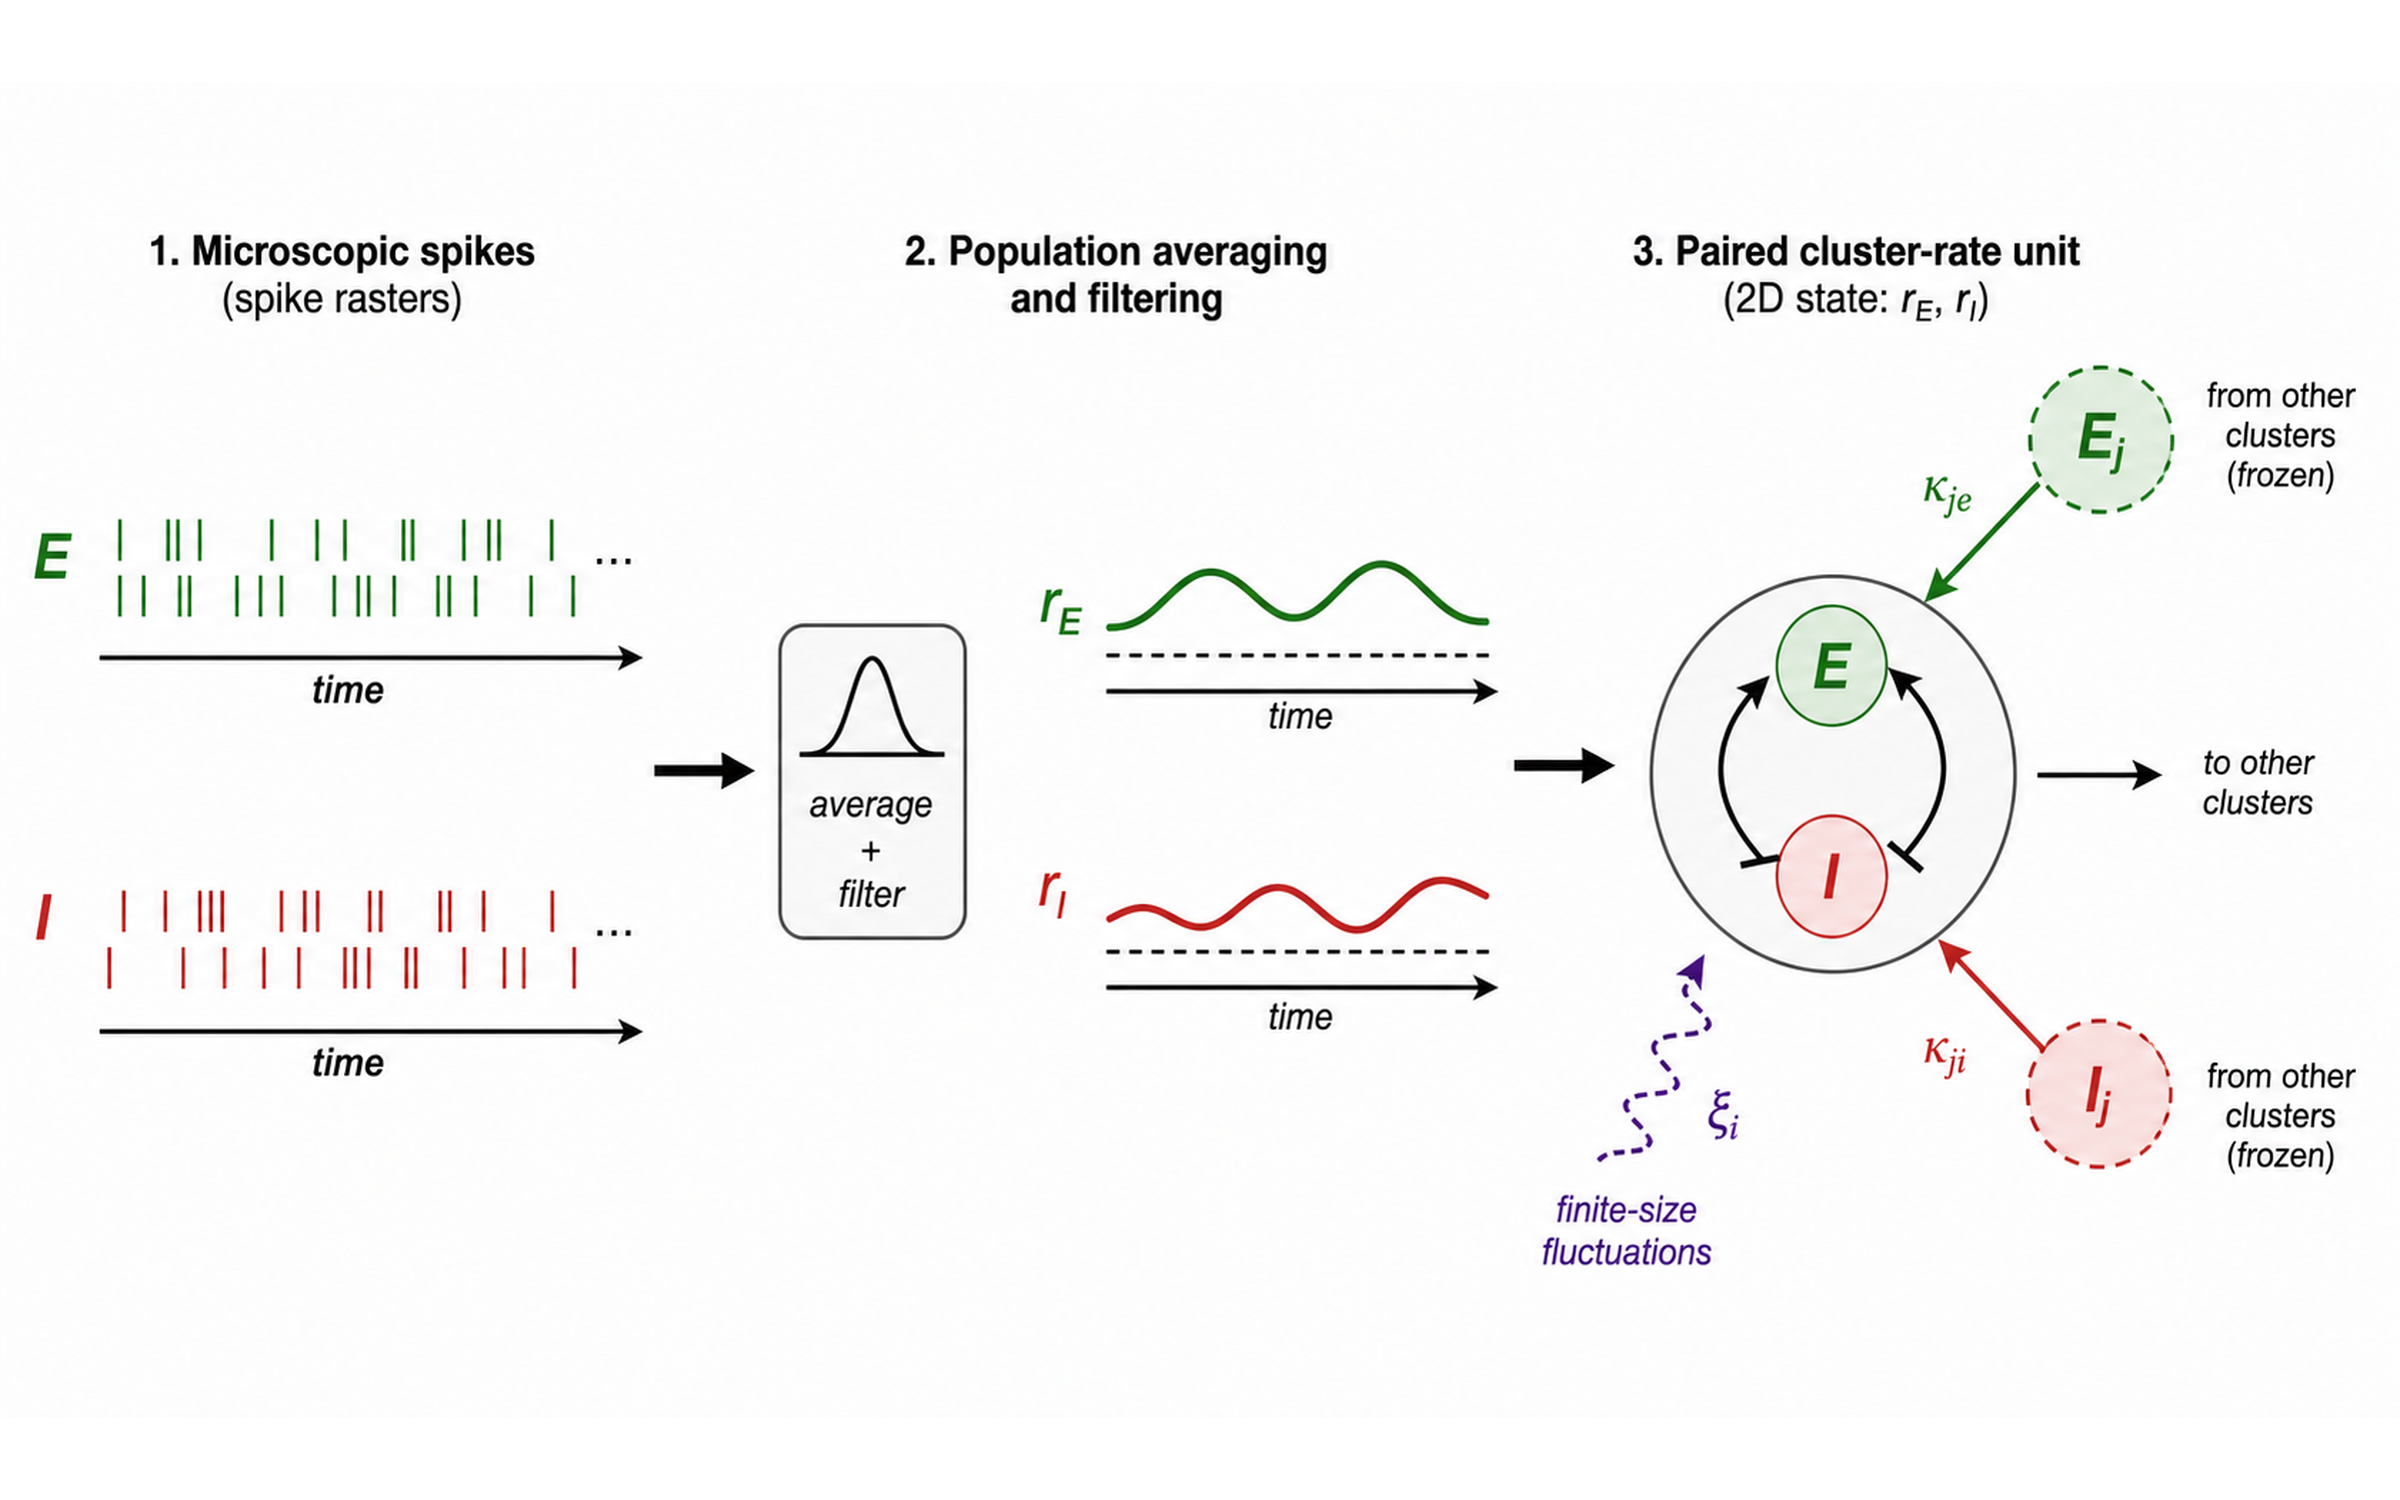
\includegraphics[width=0.92\textwidth]{figures/imagegen/ch08-cluster-rate-unit-img.png}
    \caption{From paired spiking populations to a cluster-rate unit. Microscopic E and I spike trains are averaged and filtered into the two mesoscale variables $r_a^E(t)$ and $r_a^I(t)$. Their effective dynamics combine strong within-pair coupling, frozen inter-pair input controlled by $\kappa$, and finite-size fluctuations with amplitude $\xi_E=1/\sqrt{n_E}$.}
    \label{fig:ch08-cluster-rate-unit}
\end{figure}

The quenched part of the dynamics is different. It is fixed across time for a
given network realization. A useful decomposition is
\begin{equation}
    W_{ab}^{\alpha\beta}
    =
    \frac{\overline W^{\alpha\beta}}{Q_\beta}
    +
    \frac{\kappa\sigma_{\alpha\beta}^{W}}{\sqrt{Q_\beta}}\,
    G_{ab}^{\alpha\beta},
    \qquad a\ne b,
    \label{eq:ch08-quenched-decomposition}
\end{equation}
where \(Q_\beta\) is the number of source clusters of type \(\beta\) and
\(G_{ab}^{\alpha\beta}\) has zero mean and order-one variance. The
\(1/Q_\beta\) mean scaling gives an order-one row sum, while the
\(1/\sqrt{Q_\beta}\) disorder scaling gives an order-one quenched variance after
summing over many source clusters. The parameter \(\kappa\) measures
inter-cluster heterogeneity. It may come from random weights, random
connectivity, or both. Unlike \(\xi_\alpha\), it does not vanish merely because
each cluster contains more neurons.

\section{Finite Size and Quenched Variability}
\label{sec:ch08-finite-vs-quenched}

The main conceptual distinction is between noise that is resampled in time and
disorder that is frozen into the circuit. Finite-size variability is caused by
the fact that a population rate is estimated from finitely many spikes. It is
well modeled as a dynamic fluctuation whose amplitude scales like
\(\xi_\alpha=1/\sqrt{n_\alpha}\). Quenched variability is caused by the particular
inter-cluster weights or connections. It is a property of the network instance.

This distinction is visible in the input variance. For block-shared disorder,
the clean object is the aggregated mesoscale coupling
\(W_{ab}^{\alpha\beta}\), not the variance of independent microscopic
synapses. For fixed cell indegree, \(W_{ab}^{\alpha\beta}\) is the effective
population coupling obtained after summing the selected synapses from
population \((b,\beta)\) into a representative target neuron in
\((a,\alpha)\). For dense blocks it is proportional to
\(n_\beta J_{i_a^\alpha,j_b^\beta}\). If the same quenched multiplier is shared
by all neurons in a source-target block, its variance enters through
\(W_{ab}^{\alpha\beta}\) as a block-level random variable.

Conditional on slowly varying rates, the quenched contribution to the input
\(u_a^\alpha=\sum_{\beta}\sum_{b\ne a}W_{ab}^{\alpha\beta}r_b^\beta\) is
\begin{equation}
    \operatorname{Var}_{\kappa}(u_a^\alpha)
    =
    \sum_{\beta}
    \sum_{b\ne a}
    \operatorname{Var}\!\left(W_{ab}^{\alpha\beta}\right)
    \left(r_b^\beta\right)^2 .
    \label{eq:ch08-aggregated-quenched-variance}
\end{equation}
Using the normalized decomposition in
\cref{eq:ch08-quenched-decomposition} and homogeneous rates
\(r_b^\beta=r_\beta\), this gives
\begin{equation}
    \operatorname{Var}_{\kappa}(u_a^\alpha)
    =
    \kappa^2
    \sum_{\beta}
    \frac{Q_\beta-1}{Q_\beta}
    \left(\sigma_{\alpha\beta}^{W}\right)^2
    r_\beta^2
    \approx
    \kappa^2
    \sum_{\beta}
    \left(\sigma_{\alpha\beta}^{W}\right)^2
    r_\beta^2 .
    \label{eq:ch08-normalized-quenched-variance}
\end{equation}
The \(1/\sqrt{Q_\beta}\) normalization is what keeps this term finite as the
number of source clusters grows. A formula proportional to
\(n_\beta\operatorname{Var}(J)r_\beta\) would instead describe independent
synapse-level shot noise or independent neuron-level weight disorder, not a
single multiplier shared by an entire source-target cluster pair.

Finite-size fluctuations enter through the empirical rate emitted by each
source cluster. Schematically, if
\(\operatorname{Var}(\delta r_b^\beta)\propto c_\beta r_\beta/n_\beta\), then
\begin{equation}
    \operatorname{Var}_{\xi}(u_a^\alpha)
    \approx
    \sum_{\beta}
    \sum_{b\ne a}
    \mathbb{E}\!\left[
      \left(W_{ab}^{\alpha\beta}\right)^2
    \right]
    \frac{c_\beta r_\beta}{n_\beta}.
    \label{eq:ch08-finite-size-input-variance}
\end{equation}
The constants \(c_\beta\) absorb the point-process, binning, filtering, and
gain conventions. With the same mesoscale normalization, this term scales like
\(1/n_\beta\), while the quenched term in
\cref{eq:ch08-normalized-quenched-variance} does not.

The diagnostic decomposition is therefore
\begin{equation}
    \operatorname{Var}(\delta u_a^\alpha)
    \approx
    \kappa^2
    \sum_{\beta}
    \left(\sigma_{\alpha\beta}^{W}\right)^2r_\beta^2
    +
    \sum_{\beta}
    \frac{c_{\alpha\beta}r_\beta}{n_\beta}.
    \label{eq:ch08-variance-decomposition}
\end{equation}
The first term is present because different cluster pairs have different fixed
aggregate couplings. The second term is present because a finite cluster emits
a noisy empirical spike count.

\Cref{eq:ch08-variance-decomposition} should be read as a diagnostic,
not as a complete dynamical theory. If switching disappears as \(N_c\) grows,
then it was likely driven by the second term. If switching survives after the
second term vanishes, the mechanism must live in the quenched mesoscale
dynamics.

\begin{figure}[t]
    \centering
    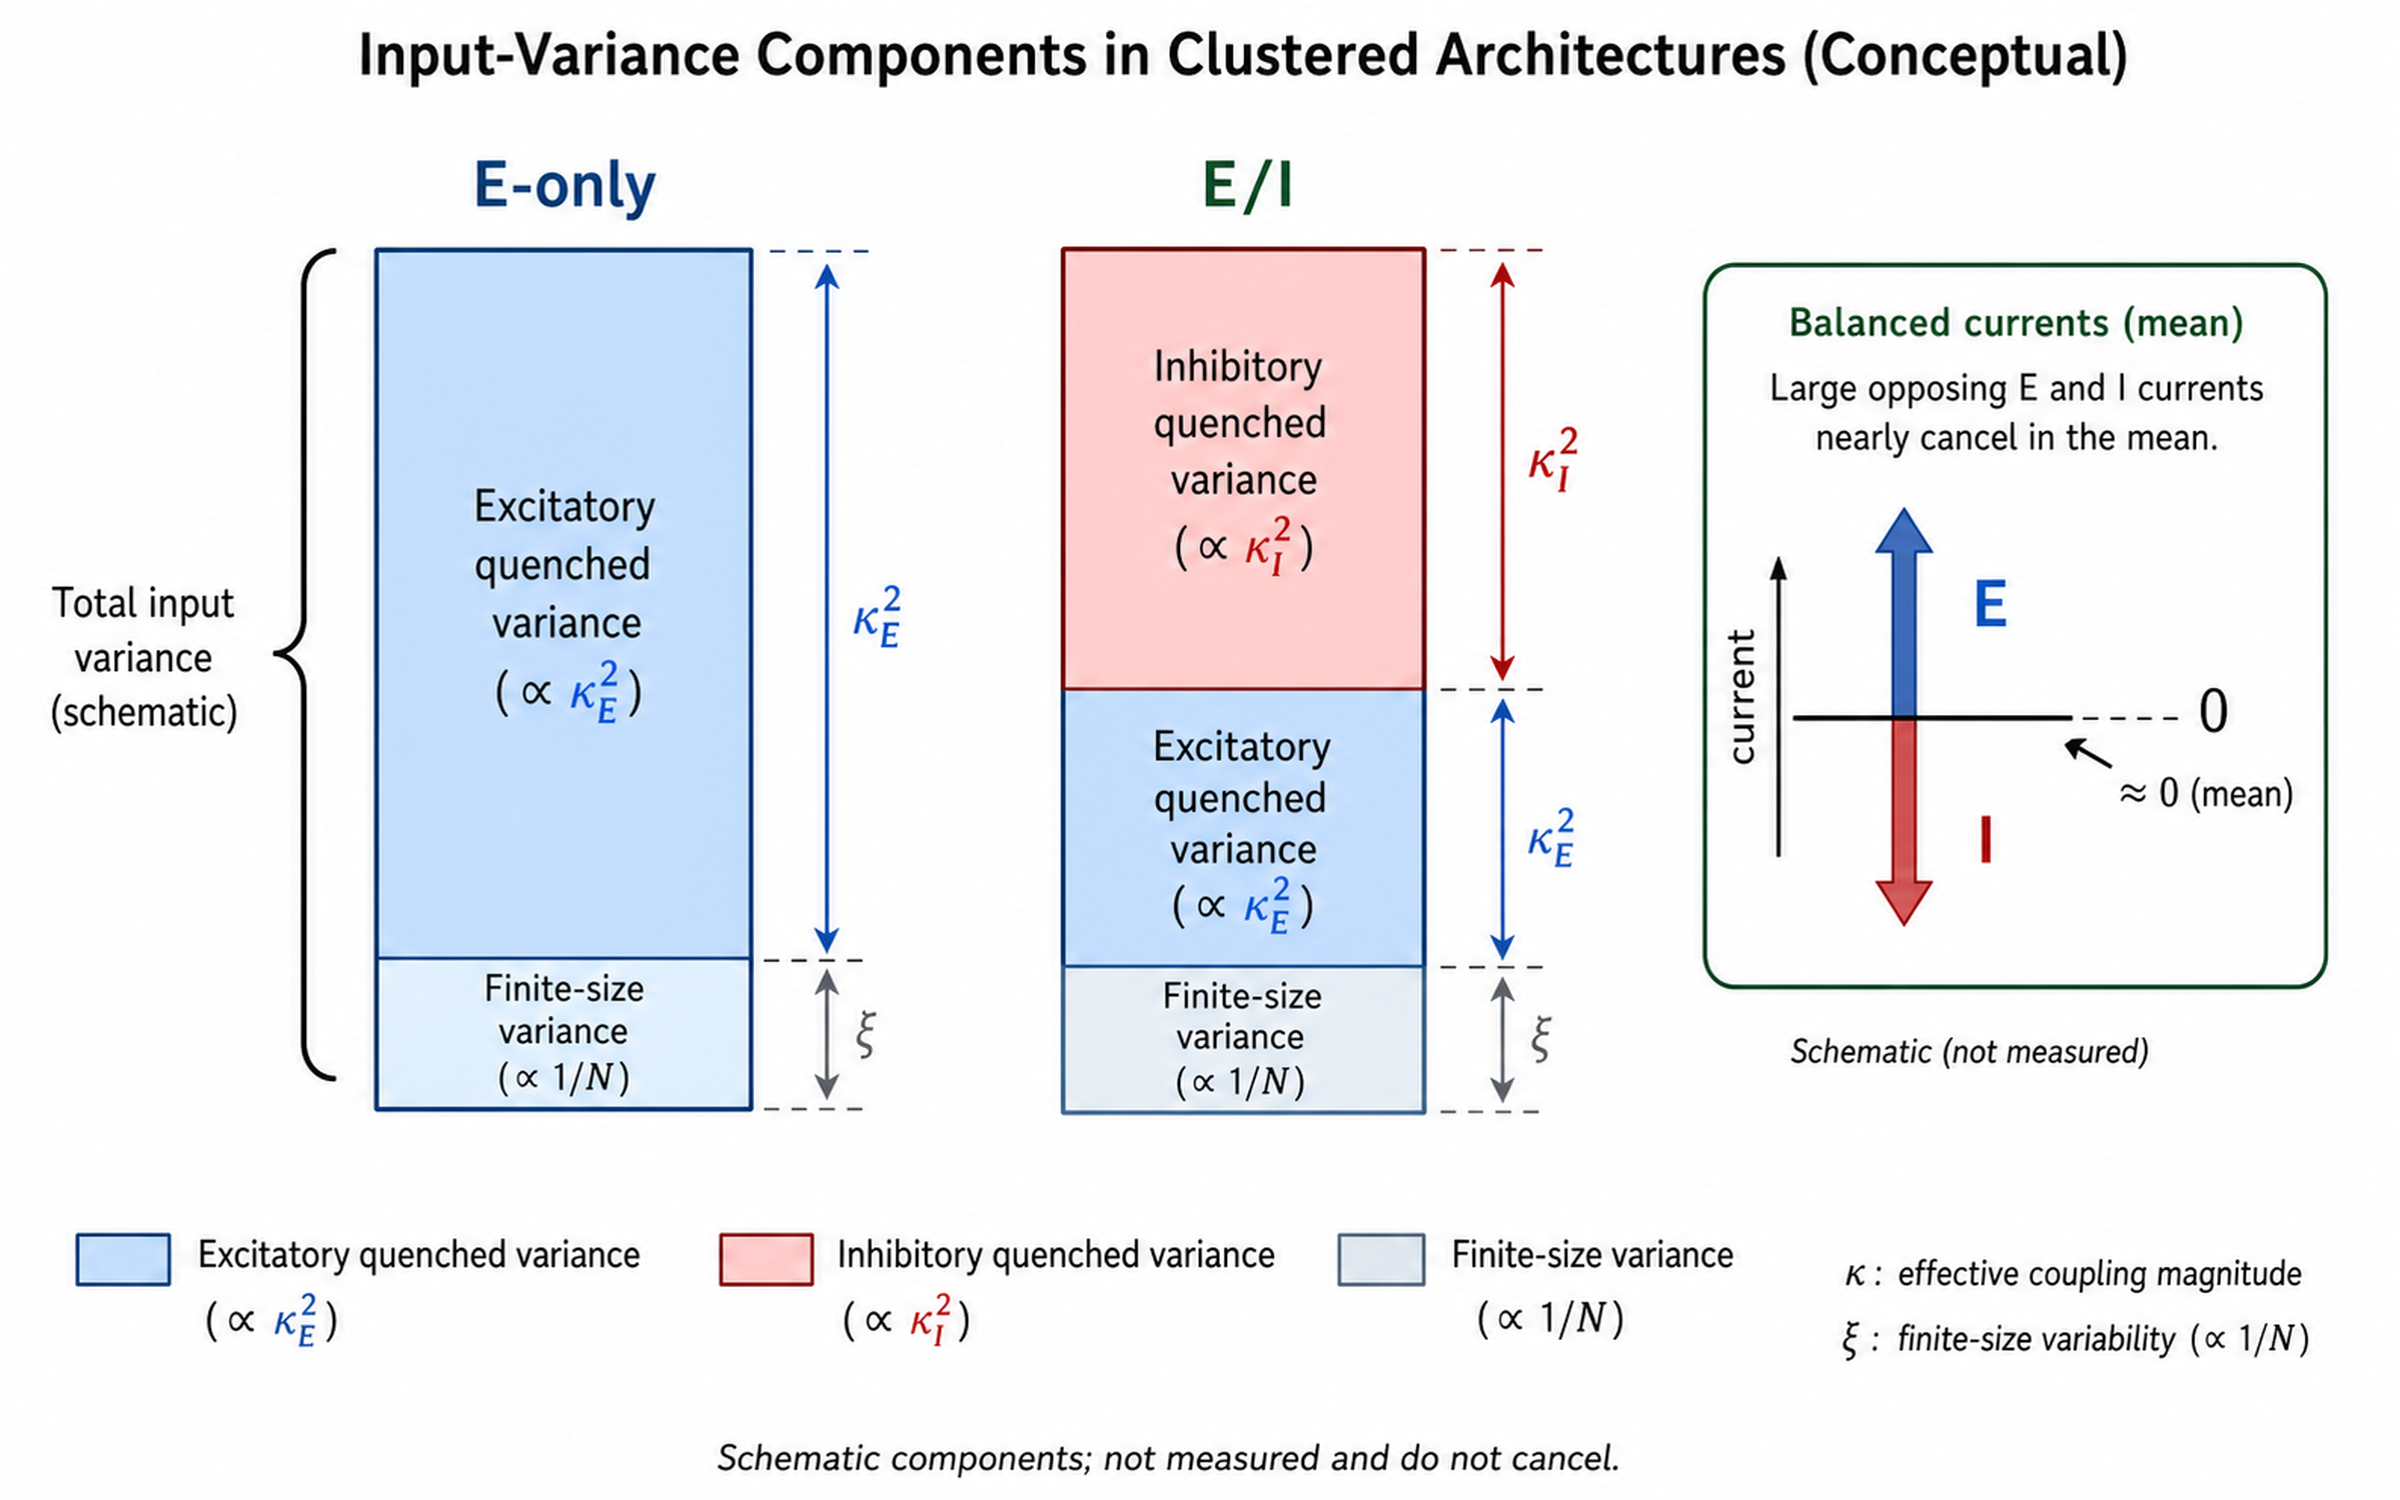
\includegraphics[width=0.84\textwidth]{figures/imagegen/ch08-quenched-amplification-img.png}
    \caption{In an inhibition-stabilized E/I network, inhibitory weights can be
    much larger in magnitude than excitatory weights. Because variance depends
    on squared coupling strength, inter-cluster heterogeneity in inhibitory
    structure can dominate the quenched input variance. This amplification is
    absent or much weaker in an E-only clustered architecture with homogeneous
    inhibition.}
    \label{fig:ch08-quenched-amplification}
\end{figure}

\section{Erdos-Renyi Variability at Two Levels}
\label{sec:ch08-er-variability}

Quenched variability does not require Gaussian-distributed weights. It can also
come from Erdos-Renyi connectivity. There are two distinct versions, and they
should not be confused.

\paragraph{Neuron-level Erdos-Renyi variability.}
Connections between individual neurons are random:
\begin{equation}
    \Pr\!\left(J_{i_a^\alpha,j_b^\beta}\ne 0\right)=p_{\alpha\beta}.
    \label{eq:ch08-neuron-er}
\end{equation}
Even if all nonzero weights have the same amplitude, each postsynaptic
population receives a random count of presynaptic spikes. The input variance
then has separate contributions from between-cluster connectivity,
within-cluster connectivity, and finite population sampling. Schematically,
\begin{equation}
\begin{aligned}
    \operatorname{Var}(I_\alpha)
    &=
    \sum_{\beta}
    \sum_{b\ne a}
    n_\beta
    p_{\alpha\beta}(1-p_{\alpha\beta})
    \left(J_{i_a^\alpha,j_b^\beta}\right)^2 r_\beta
    \\
    &\quad+
    \sum_{\beta}
    n_\beta
    p_{\alpha\beta}(1-p_{\alpha\beta})
    \left(J_{i_a^\alpha,j_a^\beta}\right)^2 r_\beta
    +
    \frac{c_\alpha r_\alpha}{n_\alpha}.
\end{aligned}
\label{eq:ch08-neuron-er-variance}
\end{equation}

\paragraph{Cluster-level Erdos-Renyi variability.}
Entire cluster pairs may be connected or disconnected:
\begin{equation}
    \Pr\!\left(\Gamma_{ab}^{\alpha\beta}=1\right)=p_{\mathrm{cl}}.
    \label{eq:ch08-cluster-er}
\end{equation}
If \(\Gamma_{ab}^{\alpha\beta}=1\), the corresponding populations can be fully
connected or have a prescribed fixed in-degree pattern. This produces a
stronger mesoscale form of disorder because the random variable is shared by
all neurons in the source-target population pair. The cluster pair is either a
present channel or an absent channel.

Both forms can be summarized by \(\kappa\), but their dynamics can differ. A
cluster-level missing inhibitory projection can change the effective vector
field of an entire rate unit. A neuron-level missing synapse is more easily
averaged away unless the scaling is chosen to keep its variance finite.

\section{Why E/I Networks Amplify Quenched Disorder}
\label{sec:ch08-ei-amplification}

Balanced networks cancel large excitation against large inhibition in the mean.
Variance does not cancel in the same way. If inhibitory currents are strong,
then heterogeneity in inhibitory projections can produce a large variance even
when the mean input remains balanced. In the variance expression
\begin{equation}
    \sum_{\beta}
    \pi_\beta
    (\sigma_{\alpha\beta}^{\mathrm{het}})^2
    j_{\alpha\beta}^2 r_\beta
    =
    \pi_E
    (\sigma_{\alpha E}^{\mathrm{het}})^2
    j_{\alpha E}^2 r_E
    +
    \pi_I
    (\sigma_{\alpha I}^{\mathrm{het}})^2
    j_{\alpha I}^2 r_I,
    \label{eq:ch08-ei-variance-terms}
\end{equation}
the inhibitory term uses \(j_{\alpha I}^2\). Its sign no longer matters. In an
inhibition-stabilized regime, effective inhibitory couplings can be larger than
effective excitatory couplings, so the inhibitory contribution to quenched
variability can dominate.

This is the mechanistic reason paired E/I clusters are not just E clusters with
extra labels. In an E-only clustered network with homogeneous inhibition, the
quenched mesoscale disorder is largely excitatory. In a paired E/I network,
randomness in inhibitory structure changes the gain, competition, and
disinhibition between cluster pairs. A small fixed difference in which
inhibitory cluster suppresses which excitatory cluster can push the effective
cluster-level vector field across a stability boundary.

\section[Qualitative Trace Examples: Nc=107 and Nc=250]{Qualitative Trace Examples: \(N_c=107\) and \(N_c=250\)}
\label{sec:ch08-trace-examples}

The roadmap contrasts population-rate traces for smaller and larger clusters,
for example \(N_c=107\) and \(N_c=250\) neurons per cluster. The important
lesson is not the exact visual appearance of those traces. It is the scaling
question they pose.

For \(N_c=107\), the finite-size amplitude \(\xi_E\) is relatively large. One
expects population traces to show visibly irregular activation and deactivation
events because empirical cluster rates are noisy. A transient high-rate episode
could be a genuine mesoscale event, or it could be a noise-driven escape from a
metastable basin.

For \(N_c=250\), \(\xi_E\) is smaller. If the same style of switching remains with
similar timescale, the case for a quenched mesoscale mechanism becomes
stronger. If switching slows dramatically or disappears, the case for
finite-size destabilization becomes stronger. These trace examples therefore
motivate the diagnostics in Chapter~\ref{ch:diagnosing-multistability-chaos}:
network-size scaling, perturbation recovery, autocorrelation shape, and
Lyapunov exponents.

\section{Chapter Summary}
\label{sec:ch08-summary}

An E/I clustered network consists of paired excitatory and inhibitory clusters.
The relevant mesoscale state of cluster \(a\) is
\((r_a^E,r_a^I)\), not just an excitatory firing rate. Tilo's notation
separates excitatory cluster strength \(J_E^+\), inhibitory cluster strength
\(J_I^+=1+R_J(J_E^+-1)\), and the compensating depression factors
\(J_E^-,J_I^-\). Finite-size noise is controlled by
\(\xi_E=1/\sqrt{n_E}=(\gamma N_c)^{-1/2}\) at fixed E/I fraction. Quenched
inter-cluster variability is controlled by \(\kappa\), which may arise from
random weights, neuron-level Erdos-Renyi connectivity, or cluster-level
Erdos-Renyi connectivity. In paired E/I networks, inhibitory structure can
strongly amplify quenched disorder because variance squares the large
inhibitory couplings instead of canceling them.

The next chapter turns this architecture into an empirical and mathematical
diagnostic problem: how can we tell whether observed switching is finite-size
multistability or deterministic mesoscopic chaos?
